\chapter{Evaluation and Discussion}
\label{chapter:Evaluation}

\section{Evaluation and Benchmarking}

\subsection{Correctness}

\subsubsection{Tricky}

We adapted the \lstinline|Tricky| example code Christensen et al. created for their implementation, which can be seen in Listing \ref{lst:tricky}.

We create the grammar starting at the node representing the variable reference \lstinline|res| in line \ref{lst:tricky:sout}.
After the regular approximation the resulting grammar contains 51 nonterminals and 59 productions.
The difference to the corresponding grammar Christensen et al. created stems from differences in the definition and implementation of the data flow graph.


The \ac{nfa} created from the grammar contains 28 states and 40 transitions, of which 27 are $\epsilon$ transitions, and is to large to display in this thesis.
The \acp{nfa} created using Nederhofs algorithm in general often have unnecessary states and transitions, like chains of states only connected with $\epsilon$ transitions.
With a length of 622 characters, the regular expression we obtain is more complex than necessary. However it accepts the correct language described with the expression \Verb|\(*<int>([+*]<int>\))*| by Christensen et al. \cite{brics}, where \Verb|<int>| abbreviates the expression \Verb@0|(-?[1-9][0-9]*)@. Note that Christensen et al. only create automata and not regular expressions, so this expression is just to describe their created automaton. How their automaton compares to ours is unclear, as they only share this description of the language.

Also note that our implementation escapes literals by surrounding them with the special characters \lstinline|\Q| and \lstinline|\E|, which adds 120 characters compared to escaping using a backslash.
To increase readability we use the \lstinline|<int>| abbreviation and replace the \lstinline|\Q\E| esape characters with single backslashes in the following regular expressions.

Like mentioned in Section \ref{sec:nfa2regex}, converting the \ac{nfa} into an equivalent \ac{dfa} significantly improves the result. The corresponding regular expression for this \ac{dfa}, which can be seen in Figure \ref{fig:eval:tricky:dfa}, is 
\begin{Verbatim}[breaklines=true, breakanywhere=true]
(((\((\()*(<int>)|<int>)(\*|\+))(((<int>)\))(\*|\+))*((<int>)\)))|(\((\()*(<int>)|<int>)
\end{Verbatim}

Minimizing the created \ac{dfa} gives the automaton in Figure \ref{fig:eval:tricky:dfamin}, which is transformed to the regular expression \Verb@(\()*<int>((\*|\+)<int>\))*@.

As Christensen et al. mention, this expression is a good result, but by distinguishing the two calls to the \lstinline|bar| method, an even more precise expression could be obtained \cite{brics}. Due to the given properties of the \ac{cpg} creation, this is currently not an option for our implementation.

\begin{figure}
	\begin{tikzpicture}[
		every initial by arrow/.style = {
			thick,-stealth
		}]
		\node (q0) [state, initial, initial where=left,
		initial text = {}] {$q_0$};
		\node (q1) [state, above right = of q0] {$q_1$};
		\node (q2) [state, accepting, below right = of q1] {$q_2$};
		\node (q3) [state, right = 2cm of q2] {$q_3$};
		\node (q4) [state, above right = of q3] {$q_4$};
		\node (q5) [state, accepting, below right = of q4] {$q_5$};
		\path [-stealth, thick]
		(q0) edge[bend left] node[above left] {(}   (q1)
		(q1) edge [loop above] node[above] {(}   (q1)
		(q0) edge node[above] {<int>}   (q2)
		(q1) edge[bend left] node[above right] {<int>}   (q2)
		(q2) edge[bend right] node[above] {+}   (q3)
		(q2) edge[bend left] node[below] {*}   (q3)
		(q3) edge[bend left] node[above left] {<int>}   (q4)
		(q4) edge[bend left] node[above right] {)}   (q5)
		(q5) edge[bend left] node[above] {+}   (q3)
		(q5) edge[bend right] node[below] {*}   (q3);
	\end{tikzpicture}
	\caption{\ac{dfa} for \lstinline|Tricky| example}
	\label{fig:eval:tricky:dfa}
\end{figure}

\begin{figure}
	\begin{tikzpicture}[
		every initial by arrow/.style = {
			thick,-stealth
		}]
		\node (q0) [state, initial, initial where=left,
		initial text = {}] {$q_0$};
		\node (q1) [state, accepting, right = of q0] {$q_1$};
		\node (q2) [state, below right = of q1] {$q_2$};
		\node (q3) [state, above right = of q1] {$q_3$};
		\path [-stealth, thick]
		(q0) edge [loop above] node[above] {(}   (q0)
		(q0) edge node[above] {<int>}   (q1)
		(q1) edge[bend right] node[above] {+}   (q2)
		(q1) edge[bend left] node[below] {*}   (q2)
		(q2) edge[bend right] node[right] {<int>}   (q3)
		(q3) edge[bend right] node[above left] {)}   (q1);
	\end{tikzpicture}
	\caption{Minimal \ac{dfa} for \lstinline|Tricky| example}
	\label{fig:eval:tricky:dfamin}
\end{figure}


\begin{lstlisting}[float, escapechar=|, numbers=right, caption=Tricky example, label=lst:tricky, captionpos=b, basicstyle=\small]
public class Tricky{
	String bar(int n, int k, String op) {
		if (k==0) {
			return "";
		}
		return op+n+"]"+bar(n-1,k-1,op)+"";
	}
	String foo(int n) {
		String b = "";
		if (n<2) {
			b = b + "(";
		}
		for (int i=0; i<n; i++){
			b = b + "(";
		}
		String s = bar(n-1,n/2-1,"*");
		String t = bar(n-n/2,n-(n/2-1),"+");
		return b+n+(s+t).replace(']',')');
	}
	public static void main(String args[]) {
		int n = new Random().nextInt();
		String res = new Tricky().foo(n);
		System.out.println(res); |\label{lst:tricky:sout}|
	}
}
\end{lstlisting}

\subsubsection{Juliet}

We also analyzed some of the test cases provided by the Juliet Java test suite\footnote{https://samate.nist.gov/SARD/test-suites/111}. The Test Suite is created by the National Security Agency’s (NSA) Center for Assured Software (CAS) and specifically designed to assess the capabilities of static analysis tools.

The test cases each target one type of flaw corresponding to a specific CWE\footnote{https://cwe.mitre.org} entry. All test cases we chose, target SQL-Injection vulnerabilities described in CWE-89, as these are flaws, where strings and string operations are the relevant points, while also being relevant risks in real applications.

The test cases in the Juliet test suite build an SQL query \lstinline|"insert into users (status) values ('updated') where name='"+data+"'"|, where \lstinline|data| is an unsanitized string with unknown value.

The cases differ in the data flow from the source of the \lstinline|data| string and the sink, where it is passed to a database library.

For all tested cases, we obtain the regular expression \Verb@(insert into users (status) values ('updated') where name='.*')@ as a result.

While the interpretation and analysis of the obtained expressions is out of scope for this thesis, it is clear that this result exposes a security risk, because an injection string can be inserted as a value for \Verb@.*@.

\subsection{Performance}

In the following section all mentioned averages are truncated averages, which means that before calculating the average, first the highest $n\%$ and the lowest $n\%$ of values are discarded. This is done to eliminate the effect of statistical outliers, which are common in software benchmarks. Such outliers are e.g. caused by unpredictable CPU scheduling and optimization. For example when running our benchmarks using JUnit tests, the first test case had the highest durations for all steps including grammar creation, approximation and automaton creation by a factor of 10-20 for some inputs. This effect occurred even when repeatedly testing the same input.

\subsubsection{Tricky}

Consider the Figures \ref{fig:eval:plot:tricky} and \ref{fig:eval:plot:trickyDFA}. 
The plots show the durations of each step in the process from \ac{cpg} to regular expression. 
In the second plot, we additionally transform the created \ac{nfa} to a \ac{dfa} before we create the regular expression, whereas in the first plot, the \ac{nfa} is converted directly. As visualized by this plot, the \ac{dfa} creation adds an additional 300 $\mu s$ to transform the automaton, but drastically reduces the time the state elimination algorithm takes to create a regular expression.

For both plots we averaged the measurements of 100 runs after we trimmed the highest and lowest 20\% of values.

\subsubsection{Juliet}

We analyzed the execution time of each hotspot of all 2224 test cases in the Juliet test suite targeting SQL Injection vulnerabilities.

Figure \ref{fig:eval:plot:juliet} shows the averaged execution times of each step, again trimmed by 20\%.
We can see, that the percentage of the total time spent on regex creation is lower compared to the plot for the Tricky example in Figure \ref{fig:eval:plot:tricky}, even without the intermediary \ac{dfa} step. This is due to the fact that the resulting automata for the Juliet test cases are very small, ranging from 2 to 4 states, compared to the 28 nodes of the Tricky \ac{nfa}.

Also note the difference in the scale of the x-axis of factor 10, which shows that the Juliet test cases are significantly faster, again due to their comparatively lower complexity.

\begin{figure}[h]
	\pgfplotsset{stackedBar/.style={
			title=Tricky,
			xbar stacked,
			width=15cm,
			axis y line*= none, axis x line*= bottom,
			xmajorgrids = true,
			xmin=0,xmax=5000,
			ytick = \empty,
			yticklabels = {},
			tick align = outside, xtick pos = left,
			bar width=6mm, y=8mm,
			enlarge y limits={abs=0.625},% 0.5 + 0.5*(y - bar width)/y [TeX.sx #47995]
	}}
	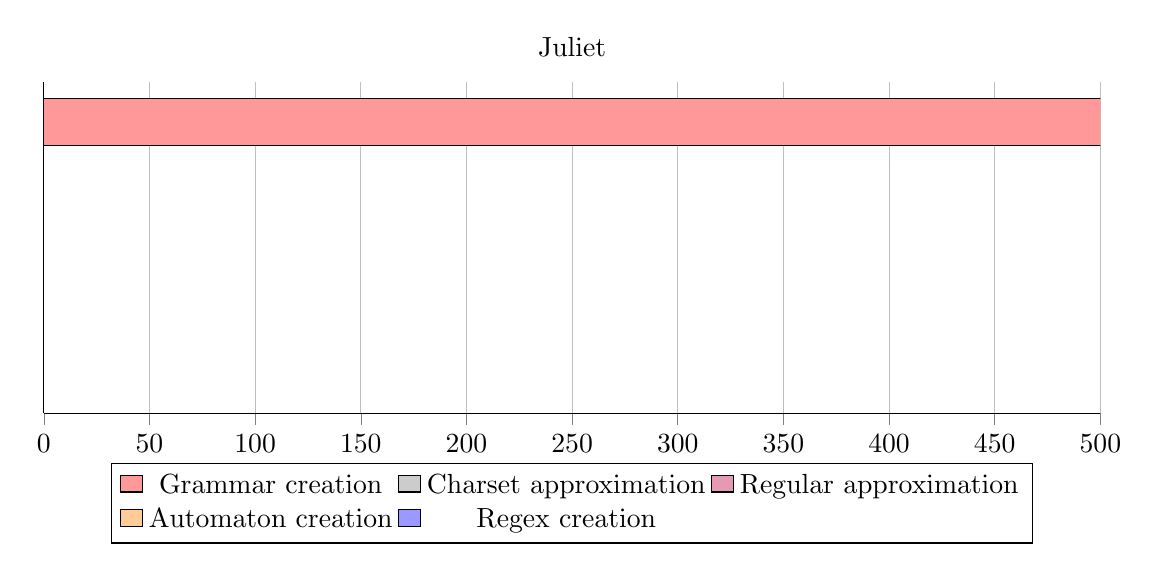
\begin{tikzpicture}
		\begin{axis}[stackedBar,legend style={area legend, at={(0.5,-0.15)}, anchor=north, legend columns=3}]
			\addplot[fill=red!40] coordinates {(1004.1666666666666, 4)};
			\addplot[fill=gray!40] coordinates {(469.55, 3)};
			\addplot[fill=purple!40] coordinates {(208.81666666666666, 2)};
			\addplot[fill=orange!40] coordinates {(609.7, 1)};
			\addplot[fill=blue!40] coordinates {(2127.1666666666665, 0)};
			\legend{Grammar creation,Charset approximation,Regular approximation,Automaton creation,Regex creation}
		\end{axis}
	\end{tikzpicture}
	\caption{Durations of Tricky example in $\mu s$}
	\label{fig:eval:plot:tricky}
\end{figure}

\begin{figure}[h!]
	\pgfplotsset{stackedBar/.style={
			title=Tricky with DFA,
			xbar stacked,
			width=15cm,
			axis y line*= none, axis x line*= bottom,
			xmajorgrids = true,
			xmin=0,xmax=5000,
			ytick = \empty,
			yticklabels = {},
			tick align = outside, xtick pos = left,
			bar width=6mm, y=8mm,
			enlarge y limits={abs=0.625},% 0.5 + 0.5*(y - bar width)/y [TeX.sx #47995]
	}}
	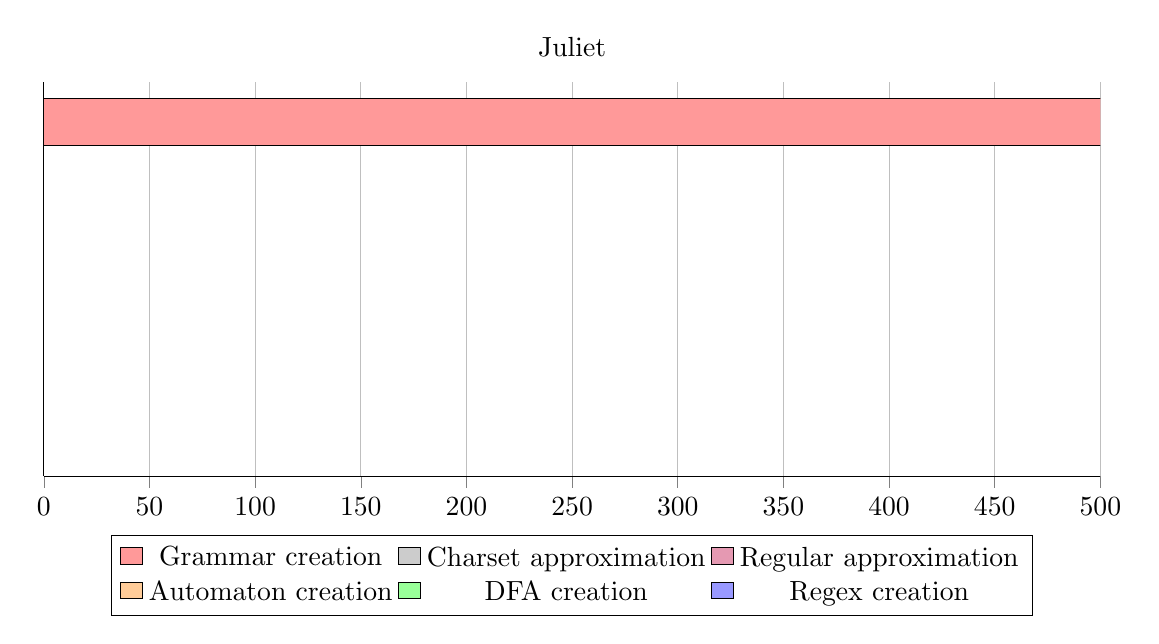
\begin{tikzpicture}
		\begin{axis}[stackedBar,legend style={area legend, at={(0.5,-0.15)}, anchor=north, legend columns=3}]
			\addplot[fill=red!40] coordinates {(944.05, 5)};
			\addplot[fill=gray!40] coordinates {(434.3333333333333, 4)};
			\addplot[fill=purple!40] coordinates {(194.41666666666666, 3)};
			\addplot[fill=orange!40] coordinates {(592.6666666666666, 2)};
			\addplot[fill=green!40] coordinates {(300.8833333333333, 1)};
			\addplot[fill=blue!40] coordinates {(326.76666666666665, 0)};
				\legend{Grammar creation,Charset approximation,Regular approximation,Automaton creation,DFA creation,Regex creation}
		\end{axis}
	\end{tikzpicture}
	\caption{Durations of Tricky example with \ac{dfa} creation in $\mu s$}
	\label{fig:eval:plot:trickyDFA}
\end{figure}

\begin{figure}
	\pgfplotsset{stackedBar/.style={
			title=Juliet,
			xbar stacked,
			width=15cm,
			axis y line*= none, axis x line*= bottom,
			xmajorgrids = true,
			xmin=0,xmax=500,
			ytick=\empty,
			yticklabels = {},
			tick align = outside, xtick pos = left,
			bar width=6mm, y=8mm,
			enlarge y limits={abs=0.625},% 0.5 + 0.5*(y - bar width)/y [TeX.sx #47995]
	}}
	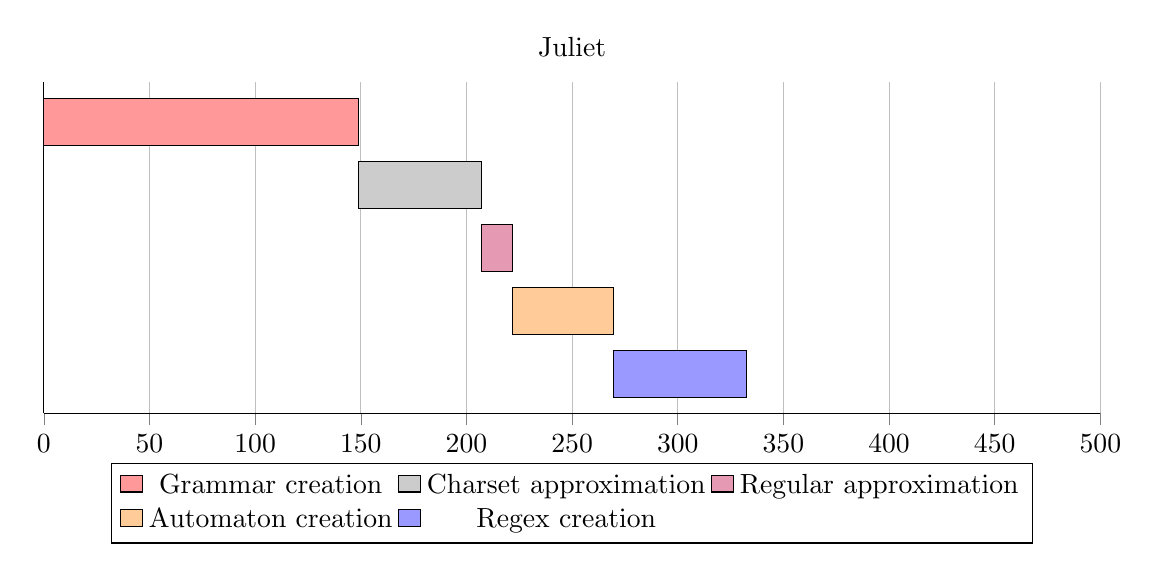
\begin{tikzpicture}
		\begin{axis}[stackedBar,legend style={area legend, at={(0.5,-0.15)}, anchor=north, legend columns=3}]
			\addplot[fill=red!40] coordinates {(148.74632967849843, 4)};
			\addplot[fill=gray!40] coordinates {(58.49117264448987, 3)};
			\addplot[fill=purple!40] coordinates {(14.738710276900205, 2)};
			\addplot[fill=orange!40] coordinates {(47.58520721055566, 1)};
			\addplot[fill=blue!40] coordinates {(63.04980486898346, 0)};
				\legend{Grammar creation,Charset approximation,Regular approximation,Automaton creation,Regex creation}
		\end{axis}
	\end{tikzpicture}
	\caption{Durations of Juliet test cases in $\mu s$}
	\label{fig:eval:plot:juliet}
\end{figure}


\section{Discussion and Future work}

\subsection{Assertions}

Our implementation currently does not try to evaluate assertions like \lstinline|s.isEmpty()| due to limitations in the creation of the \ac{cpg} we use.

Consider the example in Listing \ref{lst:assertions} where \lstinline|getSomeKnownValue()| returns some value we can analyze, which is henceforth abbreviated with the generic \lstinline|<val>|.

In our \ac{cpg} the only incoming \ac{dfg} edge of \lstinline|s|$^3$ in line \ref{lst:assertions:ifbody} is an edge from \lstinline|s|$^1$ in line \ref{lst:assertions:def}. However, there is an implicit information flow from \lstinline|s|$^2$ in line \ref{lst:assertions:condition} to \lstinline|s|$^3$, as the result of applying the \lstinline|isEmpty| operation on \lstinline|s|$^2$ influences the information we can get about \lstinline|s|$^3$. If there was a \ac{dfg} edge to the \lstinline|s|$^2$\lstinline|.isEmpty()| call from \lstinline|s|$^3$ instead of the edge from \lstinline|s|$^1$, we could include the operation in our analysis.

For example, for such an edge, we could add a new type of production comparable to the existing operation productions, from the nonterminal representing \lstinline|s|$^3$ to the one representing \lstinline|s|$^2$.

To resolve such an assertion production $A \rightarrow assertion(B)$ we could implement transformations similar to the existing operation productions. For this example, the transformation of the $isEmpty$ assertion would always return just the empty string.
In Listing \ref{lst:assertions}, we could always infer that \lstinline|s|$^3$ is empty, which is clear from the code.

For this example we currently get the regular expression \Verb@(<val>empty)|(<val>)@ as a result. 
Consider \Verb@<val>@ to be \lstinline[mathescape]@abc|$\epsilon$@, which gives us \lstinline[mathescape]@((abc|$\epsilon$)empty)|(abc|$\epsilon$)@ as our current result.
Here the first part \lstinline[mathescape]@((abc|$\epsilon$)empty)@ corresponds to the value of \lstinline|s|$^4$, which is a possible value of the analyzed \lstinline|s|$^5$ and the second part \lstinline[mathescape]@(abc|$\epsilon$)@ to the value of \lstinline|s|$^1$, which is the result if the condition evaluates to false.

With the mentioned additional \ac{dfg} edges and the described logic, we could sharpen this result.
As mentioned above, the value of \lstinline|s|$^3$ would be $\epsilon$ due to the \lstinline|isEmpty| assertion transformation and therefore \lstinline|s|$^4$ would be a concatenation of $\epsilon$ and the string \lstinline|"empty"|, so just \lstinline|empty|.

This gives us \lstinline[mathescape]@empty|(abc|$\epsilon$)@ as a result, which is more precise.

Similar transformations could also be defined for more complex assertions like \lstinline|s.length() == 1|.

However, as mentioned above, this is currently not possible because the \ac{cpg} is missing the required \ac{dfg} edges representing this implicit information flow from an assertion to subsequent variable usages.

\begin{lstlisting}[caption={Assertion Example}, label=lst:assertions, captionpos=b, float, numbers=right, escapechar=|]
String s|\textcolor{red}{$^1$}| = getSomeKnownValue(); |\label{lst:assertions:def}|
if(s|\textcolor{red}{$^2$}|.isEmpty()){ |\label{lst:assertions:condition}|
	s|\textcolor{red}{$^4$}| = s|\textcolor{red}{$^3$}| + "empty"; |\label{lst:assertions:ifbody}|
}
System.out.println(s|\textcolor{red}{$^5$}|); |\label{lst:assertions:sout}|
\end{lstlisting}

\subsection{Other Features}

Currently the \ac{cpg} does not contain \ac{dfg} edges to differentiate which field of an array is accessed in an array subscription expression like \lstinline|myArray[5]|.

Therefore, we do not further analyze values stored in arrays but rather just insert a regular expression generally describing the type stored in the array.

We mostly focused on simple strings, but in general everything we described can be applied to string builders. For example, during grammar creation, a \lstinline|ConcatProduction| is not only created for \lstinline|s1 + s2| with two strings, but also for \lstinline|sb.append(s)| with a \lstinline|StringBuilder sb| and some other string.

As this is just a proof of concept, we also implemented only a few operations on strings to showcase the approach.

\subsection{Automata Centric Approach}

We chose to provide the information we extracted only as regular expressions due to regular expressions being widely used and supported.
However, representing the information as \acp{dfa} instead of converting the automata to regular expressions has some advantages due to theoretical properties of \acp{dfa}.

Regular expression objects in most programming languages, for example Kotlin's \lstinline|Regex| object, determine, whether a given string matches the expression. With a sufficiently advanced automaton implementation more advanced checks can be made.
After analyzing a given hotspot and obtaining an automaton $M$, instead of just matching a given string as a query, the input can be a regular expression. This regular expression can then be turned into another \ac{dfa} $N$.
Since \acp{dfa} are closed under intersection and complement, we can build the \ac{dfa} $R = M \cap \overline{N}$, which accepts words that are in the language of the analysis result, but not in the language of the query expression.
Now we can check, whether $R$'s language is empty to determine, whether all strings of the query are possible values of the analyzed node. Furthermore, if $R$'s language is not empty, we can generate a word from this language as an example for a string that is a possible value of the analyzed node, but not part of the query language.
Additionally, we can check whether $M$ and $N$ are equivalent.

Since we use \acp{nfa} or optionally already \acp{dfa} as an intermediate representation, future work could increase the capabilities of our automata implementation and implement the mentioned advanced query possibilities.
\begin{comment}
\begin{itemize}
\item How did you test/evaluate your PoC?
    \begin{itemize}
    \item E.g. case studies, large-scale studies, test bench, etc.
    \item What did you do to verify results (if applicable)
    \end{itemize}
\item What did you learn from these tests? Depends on your work. E.g.
    \begin{itemize}
    \item TP/TN/FP/FN rates
    \item Performance
    \item Results of your studies
    \item Interpretation of the results, lessons learned
    \end{itemize}
\item Limitations of the approach and your implementation. Any ideas on how to fix them?
\end{itemize}

Probably 5-15 pages
\end{comment}